\documentclass{standalone}


\usepackage{tikz}
\usetikzlibrary{shapes,shadows,calc}
\usepackage{subfigure}


\begin{document}

 \begin{center}
  
  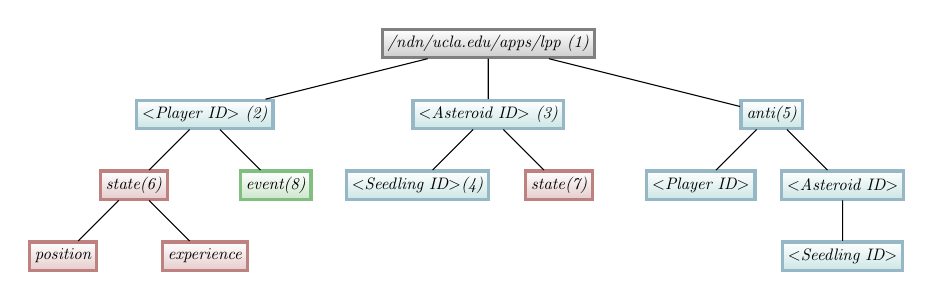
\begin{tikzpicture} [scale=0.6, transform shape,
				state/.style={
				% The shape:
				rectangle,
				% The size:
      				minimum size=6mm,
				% The border:
      				 very thick,
     				 draw=red!50!black!50,
      				% The filling:
				top color=white,
				bottom color=red!50!black!20, % and something else at the bottom % Font
				font=\itshape
    				},
				asset/.style={
				% The shape:
				rectangle,
				% The size:
      				minimum size=6mm,
				% The border:
      				very thick,draw=cyan!50!black!50,
      				% The filling:
				top color=white,
				bottom color=cyan!50!black!20, % and something else at the bottom % Font
				font=\itshape
    				},
				event/.style={
				% The shape:
				rectangle,
				% The size:
      				minimum size=6mm,
				% The border:
      				very thick,draw=green!50!black!50,
      				% The filling:
				top color=white,
				bottom color=green!50!black!20, % and something else at the bottom % Font
				font=\itshape
    				},
				default/.style={
				% The shape:
				rectangle,
				% The size:
      				minimum size=6mm,
				% The border:
      				very thick,draw=black!50,
   				top color=white,
				bottom color=black!20,
      				% The filling:
				font=\itshape
    				},
				]
    \tikzstyle{every node} = [align=center]
   % \tikzstyle{asset} = [fill=cyan!15]
   % \tikzstyle{state} = [fill=magenta!15]
   % \tikzstyle{event} = [fill=orange!15]
    \tikzstyle{level 1} = [sibling distance=60mm]
    \tikzstyle{level 2} = [sibling distance=30mm]
    \node [default] {/ndn/ucla.edu/apps/lpp (1)}
        child { node [asset] {$<$Player ID$>$ (2)} 
		child { node [state] {state(6)} 
			child { node [state] {position}}
			child { node [state] {experience}}
		}
		child { node [event] {event(8)} }
        }
        child{ node[asset] {$<$Asteroid ID$>$ (3)}
        		child{ node [asset] {$<$Seedling ID$>$(4)}}
		child { node [state] {state(7)}}
        }
         child{ node [asset] {anti(5)}
        		child { node [asset] {$<$Player ID$>$}}
		child { node [asset] {$<$Asteroid ID$>$}
			child { node [asset] {$<$Seedling ID$>$}}
		}
        }
    ;
\end{tikzpicture}


\end{center}


\end{document}